\clearpage
\section{INVERSE FUNCTIONS}\index{Function!inverse|(}\index{Inverse function|(} 
Suppose that $f:\F{R}\to \F{R}$ is continuously differentiable in an open set containing
$a$ and $f'(a)\neq 0$. If $f'(a)>0$, there is an open interval $V$ containing $a$ such that 
$f'(x)>0$ for all $x\in V$, and a similar statement holds if $f'(a)<0$. Thus $f$ is increasing
(or decreasing) on $V$, and is therefore 1-1 with an inverse function $f^{-1}$ defined on some 
open interval $W$ containing $f(a)$. Moreover it is not hard to show that $f^{-1}$ is differentiable,
and for $y\in W$ that 
\begin{align*}
    (f^{-1})'(y) = \frac{1}{f'(f^{-1}(y))}
\end{align*}

An analogous discussion in higher dimensions is much more
involved, but the result (Theorem 2-11) is very important.
We begin with a simple lemma.

\begin{lemma}
    Let $A\subset \F{R}^n$ be a rectangle and let $f:A\to \F{R}^n$ be continuously differentiable.
    If there is a number $M$ such that $|\R{D}_jf^i(x)| \le M$ for all $x$ in the interior of $A$, then 
    \begin{align*}
        \left|f(x) - f(y)\right| \le n^2M\left|x-y\right|
    \end{align*}
    for all $x, y\in A$.
\end{lemma}

\begin{proof}
    We have 
    \begin{align*}
        f^i(y) - f^i(x)
        &  = \sum_{j=1}^{n}\bigg[ f^i(y^1, \cdots, y^i, x^{j+1}, \cdots, x^n)\\
        &  \hspace*{6em} - f^i(y^1, \cdots, y^{j-1}, x^j, \cdots, x^n)\bigg]
    \end{align*}
    Applying the mean-value theorem we obtain 
    \begin{align*}
        f^i(y^1, \cdots, y^j, x^{j+1}, \cdots, x^n) 
        & - f^i(y^1, \cdots, y^{j-1}, x^j, \cdots, x^n)\\
        & \hspace*{3em} = (y^j-x^j) \cdot \R{D}_jf^i(z_{ij})
    \end{align*}
    for some $z_{ij}$, The expression on the right has absolute value less than or equal to $M\cdot |y^j-x^j|$. 
    Thus 
    \begin{align*}
        \left|f^i(y) - f^i(x)\right| 
        \le \sum_{j=1}^{n}{|y^j-x^j|\cdot M} 
        \le nM|y-x| 
    \end{align*}
    since each $|y^j - x^j| \le |y-x|$, Finally
    \begin{align*}
        |f(y) - f(x)| 
        \le \sum_{i=1}^{n}{|f^i(y) - f^i(x)|}
        \le n^2M|y-x| 
    \end{align*}
\end{proof}

\begin{theorem}[Inverse Function Theorem]\label{theorem:2-11}\index{Inverse Function Theorem}
    Suppose that $f:\F{R}^n\to \F{R}^n$ is a continuously differentiable in an open set 
    containing $a$, and $\det f'(a)\neq 0$. Then there is an open set $V$ containing $a$ and 
    a open set $W$ containing $f(a)$ such that $f:V\to W$ has a continuous inverse $f^{-1}:W\to V$ which 
    is differentiable and for all $y\in W$ satisfies 
    \begin{align*}
        (f^{-1})'(y) = \left[f'\left(f^{-1}(y)\right)\right]^{-1}
    \end{align*}
\end{theorem}

\begin{proof}
    Let $\lambda$ be the linear transformation $\R{D}f(a)$. Then $\lambda$ is non-singular,
    since $\det f'(a)\neq 0$ Now $\R{D}\left(\lambda^{-1}\circ f\right)(a) = \R{D}(\lambda^{-1})(f(a))\circ \R{D}f(a)$
    is the identity linear transformation. If the theorem is true for $\lambda^{-1}\circ f$, it is 
    clearly true for $f$. Therefore we may assume at the outset that $\lambda$ is the identity. 
    Thus whenever $f(a+h) = f(a)$, we have 
    \begin{align*}
        \frac{\left|f(a+h) - f(a) - \lambda h\right|}{|h|}
        = \frac{|h|}{|h|}
        = 1
    \end{align*}
    But 
    \begin{align*}
        \lim_{h\to 0}{\frac{\left|f(a+h) - f(a) - \lambda h\right|}{|h|}}
        = 0
    \end{align*}
    This means that we cannot have $f(x)=f(a)$ for $x$ arbitary close to, but unequal to $a$.
    Therefore there is a closed rectangle $U$ containing $a$ in its interior such that 
    \begin{enumerate}[label={\upshape(\arabic*)}]
        \item $f(x)\neq f(a)$ if $x\in U$ and $x\neq a$.\par 
            Since $f$ is continuously differentiable in 
            an open set containing $a$, we can also assume that
        \item $\det f'(x)\neq 0$ 
        \item $|\R{D}_jf^i(x) - \R{D}_jf^i(a)| < 1/2n^2$ for all $i, j$, and $x\in U$.\par 
            Note that (3) and Lemma 2-10 applied to $g(x)=f(x) - x$ imply for $x_1, x_2\in U$ that 
            \begin{align*}
                \left|f(x_1) - x_1 -\left(f(x_2) - x_2\right)\right| 
                \le \frac{1}{2}\left|x_1-x_2\right|
            \end{align*}
            Since 
            \begin{align*}
                |x_1-x_2| - |f(x_1) - f(x_2)| 
                & \le |f(x_1) - x_1 - \left(f(x_2) - x_2\right)| \\
                & \le \frac12 |x_1 - x_2|
            \end{align*}
            We obtain 
        \item $|x_1 - x_2|\le 2|f(x_1) - f(x_2)|$ for $x_1, x_2 \in U$.\par 
            Now $f(\text{boundary } U)$ is a compact set which, by (1), does not 
            contain $f(a)$ (\figref{Fig 2-3}). Therefore there is a number $d>0$ such that 
            $|f(a) - f(x)|\ge d$ for $x\in \text{boundary } U$. Let $W= \{y:|y-f(a)| < d/2\}$. 
            If $y\in W$ and $x\in \text{boundary } U$, then 
        \item $|y-f(a)| < |y-f(x)|$.\par 
            We will show that for any $y\in W$ there is a unique $x$ in
            interior $U$ such that $f(x) = y$. To prove this consider the
            \begin{figure}[!htb]
              \centering
              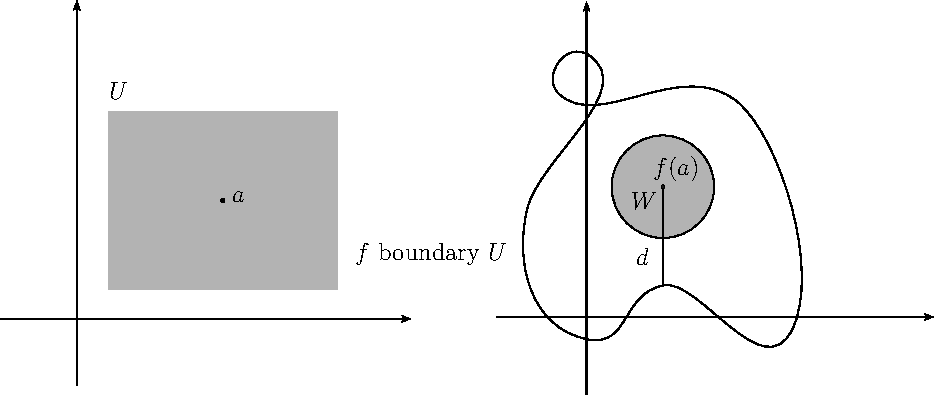
\includegraphics[width=1.45\linewidth, angle=90]{./pics/Fig2-3.pdf}
              \caption{}
              \label{Fig 2-3}
            \end{figure}
            function $g:U\to \F{R}$ defined by 
            \begin{align*}
                g(x) 
                = |y-f(x)|
                = \sum_{i=1}^{n}{\left(y^i - f^i(x)\right)^2} 
            \end{align*}
            This function is continuous and therefore has a minimum on $U$. If $x\in \text{boundary } U$, then 
            by (5), we have $g(a)< g(y)$. Therefore the minimum of $g$ does not occur on the boundary 
            of $U$. By Theorem 2-6 there is a point $x\in\text{boundary } U$ such that $\R{D}_jg(x) = 0$ for all 
            $j$, that is 
            \begin{align*}
                \sum_{i=1}^{n}{2\left(y^i - f^i(x)\right)\cdot \R{D}_jf^i(x)} = 0 \text{ for all } j 
            \end{align*}
            By (2) the matrix $(\R{D}_jf^i(x))$ has non-zero determinant. Therefore we must have $y^i - f^i(x) = 0$
            for all $i$, that is $y=f(x)$. This proves the exsitence of $x$. Uniqueness follows immediately 
            from (4). 

            If $V = \text{interior } U \cap f^{-1}(W)$, we have shown that the function 
            $f:V\to W$ has an inverse $f^{-1}:W\to V$. We can rewrite (4) as 
        \item $|f^{-1}(y_1) - f^{-1}(y_2)| \le 2|y_1 - y_2|$ for $y_1, y_2\in W$.\par 
            only the proof that $f^{-1}$ is differentiable at $y=f(x)$ with derivative 
            $\mu^{-1}$. As in the proof of Theorem 2-2, for $x_1\in V$, we have
            \begin{align*}
                f(x_1) = f(x) + \mu(x_1 - x) + \varphi(x_1 - x)
            \end{align*}
            where 
            \begin{align*}
                \lim_{x_1\to x}{\frac{\varphi(x_1 - x)}{|x_1 - x|}} = 0
            \end{align*}
            Therefore 
            \begin{align*}
                \mu^{-1}\left(f(x_1) - f(x)\right) = x_1 - x + u^{-1}\left(\varphi(x_1 - x)\right)
            \end{align*}
            Since every $y_1\in W$ is of the form $f(x_1)$ for some $x_1\in V$, this can be written.
            \begin{align*}
                f^{-1}(y_1) = f^{-1}(y) + \mu^{-1}(y_1 - y) - \mu^{-1}\left(\varphi(f^{-1}(y_1) - f^{-1}(y))\right)
            \end{align*}
            and it therefore suffices to show that
            \begin{align*}
                \lim_{y_1\to y}\frac{\left|\mu^{-1}(\varphi(f^{-1}(y_1)-f^{-1}(y)))\right|}{|y_1-y|} = 0   
            \end{align*}
            Therefore (Problem 1-10) it suffices to show that
            \begin{align*}
                \lim_{y_1\to y}\frac{\left|\varphi(f^{-1}(y_1)-f^{-1}(y))\right|}{|y_1-y|}=0
            \end{align*}
            Now 
            \begin{align*}
                \frac{\left|\varphi(f^{-1}(y_1)-f^{-1}(y))\right|}{|y_1-y|}
                \hspace*{-4pt}=\hspace*{-4pt} 
                \frac{\left|\varphi(f^{-1}(y_1)-f^{-1}(y))\right|}{|f^{-1}(y_1) - f^{-1}(y)|}
                \hspace*{-4pt}\cdot\hspace*{-4pt} 
                \frac{|f^{-1}(y_1) - f^{-1}(y)|}{|y_1-y|} 
            \end{align*}
            Since $f^{-1}$ is continuous $f^{-1}(y_1) \to f^{-1}(y)$ as $y_1\to y$. Therefore 
            the first factor approaches 0. Since, by (6), the second factor is less than 2, 
            the product also approaches 0.
    \end{enumerate}
\end{proof}

It should note that an inverse function $f^{-1}$ may exists even if $\det f'(a) = 0$. 
For example, if $f:\F{R}\to \F{R}$ is defined by $f(x) = x^3$, then $f'(0) = 0$ but $f$
has the inverse function $f^{-1}(x) = \sqrt[3]{x}$. One thing is certain however: if 
$\det f'(a) = 0$, then $f^{-1}$ cannot be differentiable at $f(a)$. To prove this note 
that $f\circ f^{-1}(x) = x$. If $f^{-1}$ were differentiable at $f(a)$, the chain rule 
would give $f'(a)\cdot (f^{-1})'(f(a)) = I$, and consequently $\det f'(a)\cdot \det(f^{-1})(f(a)) = 1$,
contradicting $\det f'(a) = 0$.
\index{Function!inverse|)} 
\index{Inverse function|)} 

\begin{problems}
    \problem[*]{Let $A \subset \F{R}^n$ be an open set and $f:A\to \F{R}^n$
        a continuously differentiable 1-1 function such that  $\det f'(x)\neq 0$
        for all $x$. Show that $f(A)$ is an open set and $f^{-1}:f(A)\to A$ is 
        differentiable. Show also that $f(B)$ is open for any open set $B\subset A$.
        }
    \problem{
        \begin{enumerate}[label={\upshape(\alph*)}]
            \item Let $f:\F{R}^2\to \F{R}$ be a continuously differentiable function.
                Show that f is not 1-1. \textit{Hint:} If, for example, $\R{D}_1f(x, y)\neq 0$
                for all $(x, y)$ in open set $A$, consider $g:A\to \F{R}^2$ defined by $g(x, y) = (f(x, y), y)$
            \item Generalize this result to the case of a continuously differentiable 
                function $f:\F{R}^n\to \F{R}^m$ with $m< n$.
        \end{enumerate}
        }
    \problem{
        \begin{enumerate}[label={\upshape(\alph*)}]
            \item If $f:\F{R}\to \F{R}$ satisfies $f'(a)\neq 0$ for all $a\in \F{R}$, show that 
                $f$ is 1-1 (on all of $\F{R}$)
            \item Defined $f:\F{R}^2 \to \F{R}^2$ by $f(x, y) = \left(\mathrm{e}^x \cos y, \mathrm{e}^x\sin y\right)$.
                Show that $\det f'(x, y)\neq 0$ for all $(x, y)$ but $f$ is not 1-1. 
        \end{enumerate}
        }
    \problem{Use the function $f:\F{R}\to \F{R}$ defined by 
        \begin{align*}
            f(x) = \left\{\begin{aligned}
                & \frac{x}{2} + x^2\sin \frac{1}{x} && x\neq 0 \\
                & 0 && x=0
            \end{aligned}\right.
        \end{align*}
        to show that continuity of the derivative cannot be eliminated from the hypothesis of Theorem 2-11.
        }
\end{problems}